\documentclass[10pt]{article}
\usepackage{icmlko}

\icmlmeta{IP 파운데이션 월드모델}{13}{좋은 선생, 나쁜 학생}{세 도메인 여섯 방향 중 넷이 건너간다 --- 게임에서 배운 것은 옮겨지지만 게임으로는 옮겨지지 않는다}

\begin{document}

\twocolumn[
\icmlheader

\begin{abstract}
노트 12는 병목을 명시했다 --- 두 도메인 세 축으로는 셀이 24개뿐이라 어떤 가설도
확정할 검정력이 없다. 세 번째 도메인을 확보했다. Steam 공개 API에서 게임 출시
482건(2006--2026)을 수집하고 같은 다섯 축을 매겼다. 먼저 구조적 결과가 하나
나왔다. \textbf{다섯 축 중 둘만 세 도메인에서 모두 관측된다} --- 매장 노출도는
게임에서 0\%, 입장 허들은 아이돌에서 0\%, 미디어 투입은 게임에서 38\%다.
공통 축은 타깃 폭과 굿즈 규모 둘뿐이다. 그 둘로 여섯 방향 전이를 검정했다.
\textbf{넷이 유의하다} --- 팝업$\to$아이돌 p=0.0013, 아이돌$\to$팝업 p=0.048,
게임$\to$팝업 p$<$0.0001, 게임$\to$아이돌 p=0.0023. 그리고 \textbf{두 축 모두
세 도메인에서 부호가 일치한다.} 실패한 둘은 방향이 아니라 목적지가 같다 ---
둘 다 게임으로 들어가는 방향이다. 도메인마다 표본을 63건으로 맞춰 300회 반복해도
같다(게임으로: 승률 35\%, 15\% / 게임에서: 80\%, 74\%). \textbf{게임은 좋은
선생이고 나쁜 학생이다.} 부수적으로 탈추세 변수의 오류를 고쳤다 --- 리뷰는 달력
시간이 아니라 출시 후 경과 시간에 누적되므로 log(경과일)로 빼야 하며, 제대로 빼자
게임으로 들어가는 전이가 더 나빠졌다.
\end{abstract}
]

\section{세 번째 도메인이 필요했던 이유}

노트 12는 증폭 가설을 세우고 확정하지 못했다. 셀이 24개뿐이었기 때문이다. 그 노트의
마지막 항목은 이랬다 --- ``도메인을 늘리는 것이 축을 늘리는 것보다 셀을 빨리 늘린다.''

게임 출시를 골랐다. IP가 대중과 만나는 접점이고, Steam 공개 API로 축과 라벨을
모두 얻을 수 있으며, 키가 필요 없다.

\begin{table}[t]
\centering\tsize
\caption{세 도메인의 구성. 표면이 전혀 다르다.}
\begin{tabular}{llr}
\toprule
도메인 & 라벨 (계수 기준) & n \\
\midrule
팝업   & 일평균 방문자 (게이트 계수) & 75 \\
아이돌 & 초동 판매량 (한터 기준) & 63 \\
게임   & 리뷰 총계 (플레이어 대리) & 482 \\
\bottomrule
\end{tabular}
\end{table}

라벨의 물리량이 다르므로 도메인 안에서 표준화한다. 검정하는 것은 절대값이 아니라
\emph{축과 결과의 관계}다.

\subsection{수집 과정에서 잡은 두 가지}

\paragraph{검색 필터가 날짜를 무시했다}
연도별로 상위작을 뽑으려고 \texttt{filter=topsellers}와 \texttt{released\_date\_range}를
함께 걸었더니 날짜 범위가 무시됐다 --- 2024년으로 걸었는데 2017년 PUBG와 2026년
팰월드가 같이 나왔다. 상위작을 통째로 받아 실제 출시일로 사후 분류하도록 고쳤고,
연도 분포가 2006--2026으로 고르게 나온다.

\paragraph{탈추세 변수가 틀렸다}
팝업과 아이돌은 달력 시간으로 시장이 커져 왔으므로 연도로 탈추세한다. 그런데
게임 리뷰는 \emph{출시일부터 누적}된다. 연도를 쓰면 부호가 반대로 나온다.

\begin{table}[t]
\centering\tsize
\caption{게임 라벨의 탈추세 변수 비교(n=482).}
\begin{tabular}{lrr}
\toprule
변수 & log 리뷰와 r & 설명력 \\
\midrule
데뷔 연도 (선형) & $-$0.583 & 34.0\% \\
\textbf{log(경과일수)} & \textbf{$+$0.690} & \textbf{47.5\%} \\
\bottomrule
\end{tabular}
\end{table}

누적은 로그 곡선이므로 형태를 맞춰야 잔차가 공정한 비교 대상이 된다. 이 수정이
결과를 바꿨다 --- 뒤에서 다룬다.

\section{다섯 축 중 둘만 공통이다}

축을 매기고 나서 예상하지 못한 결과가 먼저 나왔다.

\begin{figure}[t]
\centering
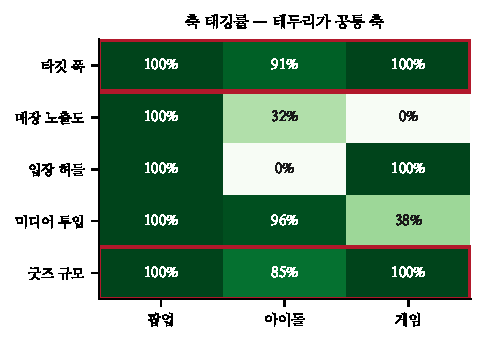
\includegraphics[width=\columnwidth]{figs/cov.pdf}
\caption{축 태깅률. 테두리 친 두 축만 세 도메인에서 모두 관측된다.}
\end{figure}

\begin{table}[t]
\centering\tsize
\caption{도메인별 축 태깅률.}
\begin{tabular}{lrrr}
\toprule
축 & 팝업 & 아이돌 & 게임 \\
\midrule
\textbf{타깃 폭}   & 100\% & 91\% & 100\% \\
\textbf{굿즈 규모} & 100\% & 85\% & 100\% \\
\midrule
미디어 투입 & 100\% & 96\% & 38\% \\
매장 노출도 & 100\% & 32\% & \textbf{0\%} \\
입장 허들   & 100\% & \textbf{0\%} & 100\% \\
\bottomrule
\end{tabular}
\end{table}

세 축이 탈락한다. 매장 노출도는 Steam이 스토어 내 노출 데이터를 공개하지 않아
게임에서 0\%다. 입장 허들은 노트 10에서 앨범 가격을 굿즈 규모로 재배치한 뒤
아이돌에서 0\%다. 미디어 투입은 게임에서 38\%인데, 표본의 퍼블리셔 대부분이
그 이전 출시작이 없기 때문이다.

이것은 실패가 아니라 제약 조건이다. 파운데이션 모델의 공유 슬롯은 \emph{모든
도메인에서 관측 가능한 축}으로만 구성될 수 있다.

\claimx{다섯 축 중 세 도메인 모두에서 관측 가능한 것은 타깃 폭과 굿즈 규모
둘뿐이다. 공유 슬롯의 개수는 축의 개수가 아니라 관측 가능성의 교집합이 정한다.}{도메인별
측정 경로를 새로 설계해 나머지 셋의 태깅률을 올릴 수 있으면 제약이 풀린다 ---
이것은 이론이 아니라 수집 과제다.}

\section{여섯 방향 중 넷이 건너간다}

공통 두 축으로 여섯 방향을 전부 검정했다. 각 방향에서 출처 도메인에서만 학습하고
대상 도메인의 라벨은 학습에 쓰지 않는다. 순열 검정은 출처 라벨을 3,000회 섞어
``전이가 없다''는 귀무가설을 직접 친다.

\begin{figure}[t]
\centering
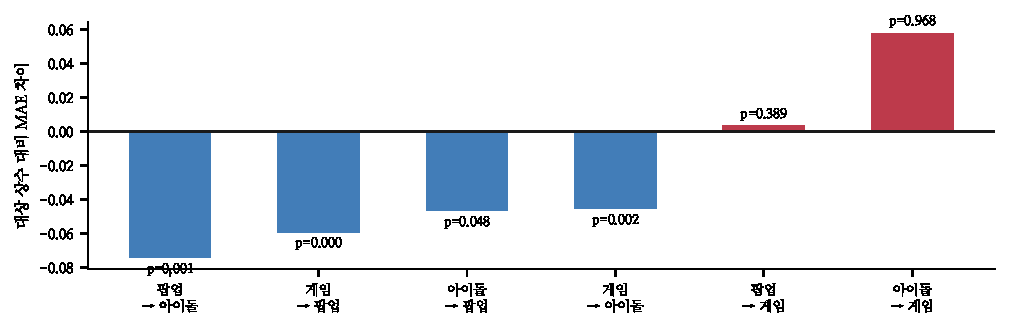
\includegraphics[width=\textwidth]{figs/six.pdf}
\caption{여섯 방향 전이. 실패한 둘은 목적지가 같다 --- 둘 다 게임으로 들어간다.}
\end{figure}

\begin{table}[t]
\centering\tsize
\caption{여섯 방향 전이. 탈추세 후, 대상 라벨 미사용.}
\begin{tabular}{lrrl}
\toprule
방향 & 차이 & 순열 p & \\
\midrule
게임 $\to$ 팝업     & $-$0.0593 & $<$0.0001 & 유의 \\
팝업 $\to$ 아이돌   & $-$0.0744 & 0.0013 & 유의 \\
게임 $\to$ 아이돌   & $-$0.0455 & 0.0023 & 유의 \\
아이돌 $\to$ 팝업   & $-$0.0467 & 0.0480 & 유의 \\
\midrule
팝업 $\to$ 게임     & $+$0.0033 & 0.3890 & 실패 \\
아이돌 $\to$ 게임   & $+$0.0576 & 0.9683 & 실패 \\
\bottomrule
\end{tabular}
\end{table}

넷이 유의하다. 그리고 실패한 둘은 무작위가 아니다 --- 둘 다 게임이 목적지다.

\section{두 축 모두 부호가 일치한다}

\begin{figure}[t]
\centering

\includegraphics[width=\columnwidth]{figs/coef.pdf}
\caption{표준화 회귀계수. 두 축 모두 세 도메인에서 양수다.}
\end{figure}

\begin{table}[t]
\centering\tsize
\caption{도메인별 표준화 회귀계수.}
\begin{tabular}{lrrr}
\toprule
축 & 팝업 & 아이돌 & 게임 \\
\midrule
타깃 폭   & $+$0.332 & $+$0.369 & $+$0.188 \\
굿즈 규모 & $+$0.211 & $+$0.435 & $+$0.074 \\
\bottomrule
\end{tabular}
\end{table}

여섯 개 계수가 전부 양수다. 대상이 넓을수록, 닿았을 때 얻을 것이 많을수록 반응이
크다 --- 팝업스토어에서도, 아이돌 데뷔에서도, 게임 출시에서도.

\claimx{타깃 폭과 굿즈 규모는 세 도메인에서 같은 부호로 작동하며, 한 도메인에서
배운 계수가 다른 도메인에서 유의하게 쓰인다(여섯 방향 중 넷). 파운데이션 월드모델의
공유 슬롯 두 개가 확정됐다.}{네 번째 도메인에서 부호가 뒤집히면 두 축은 이 세
도메인의 공통 성질이지 IP 접점 일반의 성질이 아니다.}

\section{게임은 좋은 선생이고 나쁜 학생이다}

실패한 두 방향의 원인이 표본 크기일 수 있다. 게임은 482건이고 나머지는 75건과
63건이다. 계수 추정 정밀도가 다르다.

도메인마다 63건으로 맞춰 300회 반복 부분표집했다.

\begin{figure}[t]
\centering
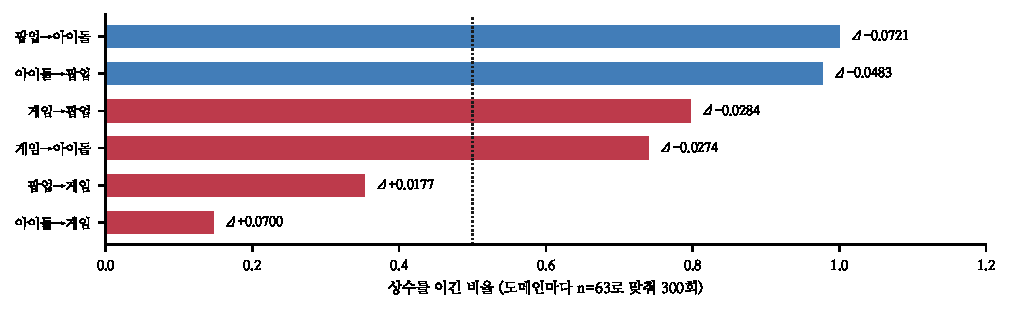
\includegraphics[width=\textwidth]{figs/bal.pdf}
\caption{표본을 맞춘 뒤에도 순서가 유지된다. 게임으로 들어가는 두 방향만 실패한다.}
\end{figure}

\begin{table}[t]
\centering\tsize
\caption{도메인마다 n=63으로 맞춰 300회 반복.}
\begin{tabular}{lrr}
\toprule
방향 & 차이 중앙 & 이긴 비율 \\
\midrule
팝업 $\to$ 아이돌   & $-$0.0721 & 100\% \\
아이돌 $\to$ 팝업   & $-$0.0483 & 98\% \\
게임 $\to$ 팝업     & $-$0.0284 & 80\% \\
게임 $\to$ 아이돌   & $-$0.0274 & 74\% \\
\midrule
팝업 $\to$ 게임     & $+$0.0177 & 35\% \\
아이돌 $\to$ 게임   & $+$0.0700 & 15\% \\
\bottomrule
\end{tabular}
\end{table}

두 가지가 동시에 보인다.

\paragraph{출처 방향은 표본 크기에 달려 있다}
게임에서 나가는 전이가 전량(n=482)에서는 p$<$0.0001인데 n=63으로 줄이면 승률
80\%로 떨어진다. 노트 10에서 세운 원리 --- 전이는 잘 측정된 쪽에서 못 측정된
쪽으로 간다 --- 가 여기서는 표본 크기의 형태로 나타난다.

\paragraph{목적지 방향은 표본 크기와 무관하다}
게임으로 들어가는 두 방향은 표본을 맞춰도 실패한다(35\%, 15\%). 게임은 대상으로서
어렵다.

\subsection{왜 게임이 어려운가}

탈추세 수정이 단서를 준다. 연도 선형으로 뺐을 때 팝업$\to$게임은 p=0.106이었는데,
log(경과일)로 제대로 빼자 p=0.389로 나빠졌다. 게임 도메인 내부 성적도
차이 $-$0.0152에서 $-$0.0098로 줄었다.

해석은 이렇다. 게임 리뷰 수 변동의 절반 가까이(47.5\%)가 출시 후 경과 시간으로
설명된다. 그것을 제거하고 남는 변동은 출시 이후에 벌어지는 일 --- 업데이트, 세일,
스트리머 노출, 입소문 --- 이 지배하며, 출시 시점의 축이 담을 수 없는 부분이다.
연도 탈추세를 썼을 때 성적이 좋아 보였던 것은 누적 곡선의 잔여분을 축이 우연히
설명한 것이었다.

\claimx{게임 도메인이 대상으로서 어려운 것은 표본 크기가 아니라 라벨의 성질
때문이다. 리뷰 총계는 출시 시점 조건이 아니라 출시 이후 수년의 누적 동역학을
반영한다.}{출시 후 첫 30일 리뷰 수만 라벨로 쓰면 출시 시점 축의 설명력이
올라가야 한다. 오르지 않으면 라벨 성질이 아니라 축 매핑이 문제다.}

\section{지금까지 확정된 것}

열세 편 끝에 파운데이션 월드모델의 골격이 이 정도로 좁혀졌다.

\begin{quote}\fontsize{9.5}{11.5}\selectfont
\textbf{공유 슬롯 2개} --- 타깃 폭, 굿즈 규모. 세 도메인에서 같은 부호,
여섯 방향 중 넷에서 유의한 전이.\\[0.4em]
\textbf{적용 조건 3개} --- 같은 부호로 작동하는가(노트 9--10), 축 측정 신뢰도가
0.79를 넘는가(노트 9), 계수 확인 뒤 이 모집단에서 축이 충분히 변하는가(노트 11--12).\\[0.4em]
\textbf{구조 제약} --- 인코더는 비선형, 헤드는 선형(노트 7). 축은 문서에서 복원되지
않으므로 측정해야 한다(노트 8).
\end{quote}

\section{한계}

\begin{itemize}[leftmargin=1.1em,itemsep=0.15em]
\item 공통 축이 둘뿐이다. 두 개의 예측변수로 이루어진 모델의 설명력은 본질적으로 작다.
\item 게임 축은 스토어 메타에서 규칙으로 유도했다. 신뢰도를 재지 않았다.
\item 게임 표본은 판매 상위작이다. 반응이 없는 게임은 표본에 없으므로 선택 편향이 있다.
\item 세 도메인 전부 한국 시장 혹은 글로벌 시장이 섞여 있다. 시장 구조를 통제하지 않았다.
\item 여섯 방향에 다중비교 보정을 하지 않았다. 본페로니를 적용하면 p=0.048인
      아이돌$\to$팝업은 유의성을 잃는다. 나머지 셋은 유지된다.
\end{itemize}

\section{다음}

\begin{enumerate}[leftmargin=1.3em,itemsep=0.15em]
\item 출시 후 30일 리뷰로 게임 라벨 재정의 --- 목적지 실패의 반증 조건.
\item 늘어난 셀로 노트 12의 증폭 가설 재검정.
\item 매장 노출도·입장 허들의 도메인별 측정 경로 설계 --- 공유 슬롯을 넷으로.
\item 두 슬롯 고정 구조의 신경망 구현과 도메인별 인코더 학습.
\end{enumerate}

\vspace{0.6em}
\hrule height 0.3pt
\vspace{0.5em}
{\footnotesize
\textbf{참고문헌}\\[0.3em]
Ben-David, S. et al. (2010). A theory of learning from different domains.
\emph{Machine Learning}, 79(1--2), 151--175.\\[0.15em]
Good, P. (2005). \emph{Permutation, Parametric, and Bootstrap Tests of Hypotheses},
3rd ed. Springer.\\[0.15em]
Maurer, A., Pontil, M., Romera-Paredes, B. (2016). The benefit of multitask
representation learning. \emph{JMLR}, 17(81), 1--32.\\[0.15em]
Standley, T. et al. (2020). Which tasks should be learned together in multi-task
learning? \emph{ICML 2020}, 9120--9132.
}

\end{document}
